% Options for packages loaded elsewhere
\PassOptionsToPackage{unicode}{hyperref}
\PassOptionsToPackage{hyphens}{url}
%
\documentclass[
]{article}
\title{Guide on reproducing BLS graphic}
\author{Xianbin Xu}
\date{8/24/2022}

\usepackage{amsmath,amssymb}
\usepackage{lmodern}
\usepackage{iftex}
\ifPDFTeX
  \usepackage[T1]{fontenc}
  \usepackage[utf8]{inputenc}
  \usepackage{textcomp} % provide euro and other symbols
\else % if luatex or xetex
  \usepackage{unicode-math}
  \defaultfontfeatures{Scale=MatchLowercase}
  \defaultfontfeatures[\rmfamily]{Ligatures=TeX,Scale=1}
\fi
% Use upquote if available, for straight quotes in verbatim environments
\IfFileExists{upquote.sty}{\usepackage{upquote}}{}
\IfFileExists{microtype.sty}{% use microtype if available
  \usepackage[]{microtype}
  \UseMicrotypeSet[protrusion]{basicmath} % disable protrusion for tt fonts
}{}
\makeatletter
\@ifundefined{KOMAClassName}{% if non-KOMA class
  \IfFileExists{parskip.sty}{%
    \usepackage{parskip}
  }{% else
    \setlength{\parindent}{0pt}
    \setlength{\parskip}{6pt plus 2pt minus 1pt}}
}{% if KOMA class
  \KOMAoptions{parskip=half}}
\makeatother
\usepackage{xcolor}
\IfFileExists{xurl.sty}{\usepackage{xurl}}{} % add URL line breaks if available
\IfFileExists{bookmark.sty}{\usepackage{bookmark}}{\usepackage{hyperref}}
\hypersetup{
  pdftitle={Guide on reproducing BLS graphic},
  pdfauthor={Xianbin Xu},
  hidelinks,
  pdfcreator={LaTeX via pandoc}}
\urlstyle{same} % disable monospaced font for URLs
\usepackage[margin=1in]{geometry}
\usepackage{color}
\usepackage{fancyvrb}
\newcommand{\VerbBar}{|}
\newcommand{\VERB}{\Verb[commandchars=\\\{\}]}
\DefineVerbatimEnvironment{Highlighting}{Verbatim}{commandchars=\\\{\}}
% Add ',fontsize=\small' for more characters per line
\usepackage{framed}
\definecolor{shadecolor}{RGB}{248,248,248}
\newenvironment{Shaded}{\begin{snugshade}}{\end{snugshade}}
\newcommand{\AlertTok}[1]{\textcolor[rgb]{0.94,0.16,0.16}{#1}}
\newcommand{\AnnotationTok}[1]{\textcolor[rgb]{0.56,0.35,0.01}{\textbf{\textit{#1}}}}
\newcommand{\AttributeTok}[1]{\textcolor[rgb]{0.77,0.63,0.00}{#1}}
\newcommand{\BaseNTok}[1]{\textcolor[rgb]{0.00,0.00,0.81}{#1}}
\newcommand{\BuiltInTok}[1]{#1}
\newcommand{\CharTok}[1]{\textcolor[rgb]{0.31,0.60,0.02}{#1}}
\newcommand{\CommentTok}[1]{\textcolor[rgb]{0.56,0.35,0.01}{\textit{#1}}}
\newcommand{\CommentVarTok}[1]{\textcolor[rgb]{0.56,0.35,0.01}{\textbf{\textit{#1}}}}
\newcommand{\ConstantTok}[1]{\textcolor[rgb]{0.00,0.00,0.00}{#1}}
\newcommand{\ControlFlowTok}[1]{\textcolor[rgb]{0.13,0.29,0.53}{\textbf{#1}}}
\newcommand{\DataTypeTok}[1]{\textcolor[rgb]{0.13,0.29,0.53}{#1}}
\newcommand{\DecValTok}[1]{\textcolor[rgb]{0.00,0.00,0.81}{#1}}
\newcommand{\DocumentationTok}[1]{\textcolor[rgb]{0.56,0.35,0.01}{\textbf{\textit{#1}}}}
\newcommand{\ErrorTok}[1]{\textcolor[rgb]{0.64,0.00,0.00}{\textbf{#1}}}
\newcommand{\ExtensionTok}[1]{#1}
\newcommand{\FloatTok}[1]{\textcolor[rgb]{0.00,0.00,0.81}{#1}}
\newcommand{\FunctionTok}[1]{\textcolor[rgb]{0.00,0.00,0.00}{#1}}
\newcommand{\ImportTok}[1]{#1}
\newcommand{\InformationTok}[1]{\textcolor[rgb]{0.56,0.35,0.01}{\textbf{\textit{#1}}}}
\newcommand{\KeywordTok}[1]{\textcolor[rgb]{0.13,0.29,0.53}{\textbf{#1}}}
\newcommand{\NormalTok}[1]{#1}
\newcommand{\OperatorTok}[1]{\textcolor[rgb]{0.81,0.36,0.00}{\textbf{#1}}}
\newcommand{\OtherTok}[1]{\textcolor[rgb]{0.56,0.35,0.01}{#1}}
\newcommand{\PreprocessorTok}[1]{\textcolor[rgb]{0.56,0.35,0.01}{\textit{#1}}}
\newcommand{\RegionMarkerTok}[1]{#1}
\newcommand{\SpecialCharTok}[1]{\textcolor[rgb]{0.00,0.00,0.00}{#1}}
\newcommand{\SpecialStringTok}[1]{\textcolor[rgb]{0.31,0.60,0.02}{#1}}
\newcommand{\StringTok}[1]{\textcolor[rgb]{0.31,0.60,0.02}{#1}}
\newcommand{\VariableTok}[1]{\textcolor[rgb]{0.00,0.00,0.00}{#1}}
\newcommand{\VerbatimStringTok}[1]{\textcolor[rgb]{0.31,0.60,0.02}{#1}}
\newcommand{\WarningTok}[1]{\textcolor[rgb]{0.56,0.35,0.01}{\textbf{\textit{#1}}}}
\usepackage{graphicx}
\makeatletter
\def\maxwidth{\ifdim\Gin@nat@width>\linewidth\linewidth\else\Gin@nat@width\fi}
\def\maxheight{\ifdim\Gin@nat@height>\textheight\textheight\else\Gin@nat@height\fi}
\makeatother
% Scale images if necessary, so that they will not overflow the page
% margins by default, and it is still possible to overwrite the defaults
% using explicit options in \includegraphics[width, height, ...]{}
\setkeys{Gin}{width=\maxwidth,height=\maxheight,keepaspectratio}
% Set default figure placement to htbp
\makeatletter
\def\fps@figure{htbp}
\makeatother
\setlength{\emergencystretch}{3em} % prevent overfull lines
\providecommand{\tightlist}{%
  \setlength{\itemsep}{0pt}\setlength{\parskip}{0pt}}
\setcounter{secnumdepth}{-\maxdimen} % remove section numbering
\usepackage{amsmath}
\ifLuaTeX
  \usepackage{selnolig}  % disable illegal ligatures
\fi

\begin{document}
\maketitle

\hypertarget{introduction}{%
\subsection{Introduction}\label{introduction}}

This R Markdown file replicates various graphics from Bureau of Labor
Statistics data. It contains specific instructions and replicable codes.

\hypertarget{running-environment}{%
\subsection{Running Environment}\label{running-environment}}

This RMD (R Markdown) file had been knitted into a PDF file for easier
reading. PDF file and R Markdown file(end with .rmd) are all included in
the directory under the same name. To reproduce the code, open the R
Markdown in RStudio, then run the whole markdown file.

To get a LaTeX file of the document, add ``keep\_tex: true'' below the
pdf\_output: line, in the header section of R Markdown. Then, knit the
whole markdown file.

Make sure the file is located in \(/\)Graphic\_Reproduction\_Folder,
with directory BLS\_Data in the same directory containing
\(/\)Graphic\_Reproduction\_Folder.

Make sure the following files are in place at BLS\_Data folder:

\begin{quote}
\begin{quote}
Employment\_By\_State.csv. It can be recreated by running
BLS\_Download\_State\_Level.R
\end{quote}
\end{quote}

The following packages are used:

\begin{Shaded}
\begin{Highlighting}[]
\FunctionTok{library}\NormalTok{(}\StringTok{"dplyr"}\NormalTok{) }\CommentTok{\# For data processing}
\FunctionTok{library}\NormalTok{(}\StringTok{"tidyr"}\NormalTok{)}
\end{Highlighting}
\end{Shaded}

use install.packages() to install if you haven't installed already. The
formatR package was used to creat tidy code chunks for easier reading.
You will NOT need it if you just do the codes in R Studio.

\hypertarget{creating-a-function-for-jobs-per-capita-scatterplot}{%
\subsection{Creating a function for jobs-per-capita
scatterplot}\label{creating-a-function-for-jobs-per-capita-scatterplot}}

Read the file.

\begin{Shaded}
\begin{Highlighting}[]
\NormalTok{Employment\_Data }\OtherTok{=} \FunctionTok{read.csv}\NormalTok{(}\StringTok{"./../BLS\_Data/Employment\_By\_State.csv"}\NormalTok{)}
\end{Highlighting}
\end{Shaded}

Here, the ../ get us to the directory containing both
Graphic\_Reproduction\_Folder and BLS\_Data.

The following function shall be used to calculate job-to-population
ratio, averaged over years, for each state. Washington DC was included,
with abbreviation DC, but Puerto Rico was not, due to it not being a
state but always being an outlier. The formula is:

\begin{center}
$$\text{job ratio growth} = \displaystyle \frac{\displaystyle \sum _{\text{ begin year of the period }} ^{\text{end year of the period}} \text{employment by year}} {\displaystyle \sum _{\text {begin year of the period}} ^{\text {End Year of the period}} \text{population by year}}$$
\end{center}

By calculating ave\_job\_ratio for two periods, we can find job ratio
growth:

job\_ratio\_growth = Ave\_job\_ratio in period 2 / Ave\_job\_ratio in
period 1

This is considered the growth of job per capita, where
\(\text{job ratio growth} < 1\) means a shrink in job per capita and
\(>1\) means an increase.

By designating two occupations, we can create a scatterplot on the
job\_ratio\_growth for two occupations, where X and Y axis each gives
refers to an occupation.

I used function instead of codes because it will give an easier time
trying to recreate same plot under different variables. The variables
used are as the following:

\begin{quote}
\begin{quote}
First\_Occupation and Second\_Occupation refers to names of occupations
on X and Y axis respectively.
\end{quote}
\end{quote}

\begin{quote}
\begin{quote}
Input\_Data refers to data frame to be used, in our case just use
Employment\_Data
\end{quote}
\end{quote}

\begin{quote}
\begin{quote}
Begin\_Year\_1 and End\_Year\_1 refers to beginning and ending year for
period 1. Beginning and Ending years are included when averaging
\end{quote}
\end{quote}

\begin{quote}
\begin{quote}
Plot = 1 if you want to get the plot. Default is 1.
\end{quote}
\end{quote}

\begin{quote}
\begin{quote}
give\_provessed\_data = 1 if you want to get processed data that was
directly used in plot function. Default is 0 (Don't return)
\end{quote}
\end{quote}

Specific technical details are included in code chunk.

\begin{Shaded}
\begin{Highlighting}[]
\NormalTok{Ratio\_Extractor }\OtherTok{=} \ControlFlowTok{function}\NormalTok{(First\_Occupation, Second\_Occupation, Input\_Data,  }
                           \AttributeTok{Begin\_Year\_1 =} \DecValTok{2009}\NormalTok{, }\AttributeTok{End\_Year\_1 =} \DecValTok{2011}\NormalTok{,}
                           \AttributeTok{Begin\_Year\_2 =} \DecValTok{2014}\NormalTok{, }\AttributeTok{End\_Year\_2 =} \DecValTok{2016}\NormalTok{,}
                           \AttributeTok{plot =} \DecValTok{1}\NormalTok{, }\AttributeTok{give\_processed\_data =} \DecValTok{0}\NormalTok{)\{}

  
\NormalTok{  temp }\OtherTok{=}\NormalTok{ Input\_Data}
\NormalTok{  temp }\OtherTok{=}\NormalTok{ temp[temp}\SpecialCharTok{$}\NormalTok{job\_type }\SpecialCharTok{==}\NormalTok{ First\_Occupation }\SpecialCharTok{|} 
\NormalTok{                temp}\SpecialCharTok{$}\NormalTok{job\_type }\SpecialCharTok{==}\NormalTok{ Second\_Occupation, ]}

  \DocumentationTok{\#\#\# This two steps includes only two occupations which we are plotting}
  
\NormalTok{  temp }\OtherTok{=}\NormalTok{ temp[temp}\SpecialCharTok{$}\NormalTok{st }\SpecialCharTok{!=} \StringTok{"PR"}\NormalTok{, ]}
  \DocumentationTok{\#\#\# Drop Puerto Rico.}
  
  
  \CommentTok{\# Categorize by job type}
\NormalTok{  temp }\OtherTok{=}\NormalTok{ temp }\SpecialCharTok{\%\textgreater{}\%} \FunctionTok{mutate}\NormalTok{(}\AttributeTok{year\_period =} \FunctionTok{case\_when}\NormalTok{(}
\NormalTok{    year }\SpecialCharTok{\textgreater{}=}\NormalTok{ Begin\_Year\_1 }\SpecialCharTok{\&}\NormalTok{ year }\SpecialCharTok{\textless{}=}\NormalTok{ End\_Year\_1 }\SpecialCharTok{\textasciitilde{}} \DecValTok{1}\NormalTok{, }\CommentTok{\#First Period}
\NormalTok{    year }\SpecialCharTok{\textgreater{}=}\NormalTok{ Begin\_Year\_2 }\SpecialCharTok{\&}\NormalTok{ year }\SpecialCharTok{\textless{}=}\NormalTok{ End\_Year\_2 }\SpecialCharTok{\textasciitilde{}} \DecValTok{2}\NormalTok{, }\CommentTok{\#Second Period}
    \ConstantTok{TRUE} \SpecialCharTok{\textasciitilde{}} \SpecialCharTok{{-}}\DecValTok{1}
    
    \DocumentationTok{\#\#\# The year is a variable in input\_data (here included as "temp"). }
    \DocumentationTok{\#\#\#It refers to the year of the data entry.}
    \DocumentationTok{\#\#\# If it is between beginning\_year\_1 and end\_year\_1, }
    \DocumentationTok{\#\#\# include it as 1, meaning it being in period 1.}
    \DocumentationTok{\#\#\# Similarly we get result for period 2.}
    
    \DocumentationTok{\#\#\# If you need to have overlap between two periods, this code unfortunately }
    \DocumentationTok{\#\#\# cannot do it.Instead you will need two variables for them.}
\NormalTok{  )) }\SpecialCharTok{\%\textgreater{}\%} \FunctionTok{filter}\NormalTok{(year\_period }\SpecialCharTok{!=} \SpecialCharTok{{-}}\DecValTok{1}\NormalTok{) }\OtherTok{{-}\textgreater{}}\NormalTok{ temp}
  
  \CommentTok{\# Having 0 or NA in any of the tot\_employment means the raw data was NOT available. }
  \CommentTok{\# Thus, we keep only those with good data.}
\NormalTok{  temp }\OtherTok{=}\NormalTok{ temp[}\SpecialCharTok{!}\NormalTok{(}\FunctionTok{is.na}\NormalTok{(temp}\SpecialCharTok{$}\NormalTok{Est\_Population) }\SpecialCharTok{|}\NormalTok{ temp}\SpecialCharTok{$}\NormalTok{tot\_employment }\SpecialCharTok{==} \DecValTok{0}\NormalTok{), ]}
  
  \CommentTok{\# Keep only needed variables. st variable stores abbreviation of states\textquotesingle{} name}
\NormalTok{  temp }\OtherTok{=}\NormalTok{ temp[, }\FunctionTok{c}\NormalTok{(}\StringTok{"st"}\NormalTok{, }\StringTok{"job\_type"}\NormalTok{, }\StringTok{"occ\_code"}\NormalTok{, }\StringTok{"tot\_employment"}\NormalTok{, }
                  \StringTok{"year"}\NormalTok{, }\StringTok{"Est\_Population"}\NormalTok{, }\StringTok{"year\_period"}\NormalTok{)]}
  
  \CommentTok{\# Group by st(state abbreviations), job, and year\_period}
\NormalTok{  temp }\OtherTok{=}\NormalTok{ temp }\SpecialCharTok{\%\textgreater{}\%} \FunctionTok{group\_by}\NormalTok{(st, job\_type, year\_period) }\SpecialCharTok{\%\textgreater{}\%}
    \FunctionTok{summarize}\NormalTok{(}\AttributeTok{ave\_ratio =} \FunctionTok{sum}\NormalTok{(tot\_employment) }\SpecialCharTok{/} \FunctionTok{sum}\NormalTok{(Est\_Population)) }\SpecialCharTok{\%\textgreater{}\%}
    \CommentTok{\# for each state{-}job{-}year period, use ave\_job\_ratio formula }
    \CommentTok{\# to find the averaged job per capita.}
    \CommentTok{\# There shouldn\textquotesingle{}t be an NA problem since they were all dropped above}
    \FunctionTok{unique}\NormalTok{()}
  
  
\NormalTok{  temp }\OtherTok{=}\NormalTok{ temp }\SpecialCharTok{\%\textgreater{}\%} \FunctionTok{pivot\_wider}\NormalTok{(}\AttributeTok{names\_from =}\NormalTok{ year\_period, }\AttributeTok{values\_from =}\NormalTok{ ave\_ratio,}
                              \AttributeTok{names\_prefix =} \StringTok{"year\_period\_"}\NormalTok{) }\SpecialCharTok{\%\textgreater{}\%}
    
    \DocumentationTok{\#\# The Pivot\_Wider part shall expand the dataset.}
    \DocumentationTok{\#\# The year\_period value would become two new variables, }
    \DocumentationTok{\#\# year\_period\_1 and year\_period\_2,}
    \DocumentationTok{\#\# and have job\_ratio of the respective period beneath it.}
    \DocumentationTok{\#\# As such, we shall have state{-}job ratio for two periods.}
    
    \FunctionTok{select}\NormalTok{(st, job\_type, year\_period\_1, year\_period\_2) }\SpecialCharTok{\%\textgreater{}\%}
    \FunctionTok{mutate}\NormalTok{(}\AttributeTok{job\_ratio\_growth =}\NormalTok{ year\_period\_2 }\SpecialCharTok{/}\NormalTok{ year\_period\_1) }\SpecialCharTok{\%\textgreater{}\%}
    
    \DocumentationTok{\#\#\# The mutate step finds the growth in the job ratio.}
    
    \FunctionTok{select}\NormalTok{(st, job\_type, job\_ratio\_growth) }\SpecialCharTok{\%\textgreater{}\%}
    
    \CommentTok{\# Keep only the three columns we need}
    
    \FunctionTok{pivot\_wider}\NormalTok{(}\AttributeTok{names\_from =}\NormalTok{ job\_type, }\AttributeTok{values\_from =}\NormalTok{ job\_ratio\_growth,}
                \AttributeTok{names\_prefix =} \StringTok{"Job Ratio Growth, "}\NormalTok{)}
  
  \DocumentationTok{\#\#\# Finally, we shall pivot again so that job\_growth\_ratios for both}
  \DocumentationTok{\#\#\# jobs are two variables.}
  \DocumentationTok{\#\#\# The plotting function does not discern different values from a variable }
  \DocumentationTok{\#\#\# but requires two variables for X and Y axis respectively.}
  
\NormalTok{  temp }\OtherTok{=} \FunctionTok{as.data.frame}\NormalTok{(temp)}
  \DocumentationTok{\#\#\# The temp here is of "group" class. It should be converted back to }
  \DocumentationTok{\#\# data frame to be used for plotting}
  
  
\NormalTok{  temp }\OtherTok{=}\NormalTok{ temp[, }\FunctionTok{c}\NormalTok{(}\StringTok{"st"}\NormalTok{, }\FunctionTok{paste}\NormalTok{(}\StringTok{"Job Ratio Growth, "}\NormalTok{, First\_Occupation, }\AttributeTok{sep =} \StringTok{""}\NormalTok{),}
                  \FunctionTok{paste}\NormalTok{(}\StringTok{"Job Ratio Growth, "}\NormalTok{, Second\_Occupation, }\AttributeTok{sep =} \StringTok{""}\NormalTok{))]}
  
  \CommentTok{\# We shall rename the variables under the occupations\textquotesingle{} names.}
  \DocumentationTok{\#\#\# In this way, we can tell the X{-}axis from the Y{-}axis.}
  \DocumentationTok{\#\#\# Note that the naming does NOT use underline but spaces. }
  \DocumentationTok{\#\#\# This is useful for plotting and plotting only.}
  \DocumentationTok{\#\#\# So we don\textquotesingle{}t bother changing the X and Y axis again.}
    
  \ControlFlowTok{if}\NormalTok{(plot }\SpecialCharTok{==} \DecValTok{1}\NormalTok{)\{}
    \DocumentationTok{\#\#\# This chunk only runs when plot is 1, which does the plotting}
    \FunctionTok{plot}\NormalTok{(}\AttributeTok{x =}\NormalTok{ temp[, }\DecValTok{2}\NormalTok{], }\AttributeTok{y =}\NormalTok{ temp[, }\DecValTok{3}\NormalTok{],}
         \AttributeTok{xlab =} \FunctionTok{colnames}\NormalTok{(temp)[}\DecValTok{2}\NormalTok{],}
         \AttributeTok{ylab =} \FunctionTok{colnames}\NormalTok{(temp)[}\DecValTok{3}\NormalTok{])}
    \FunctionTok{title}\NormalTok{(}\AttributeTok{main =} \StringTok{"Growth in Averaged Job to Population Ratio"}\NormalTok{,}
          \DocumentationTok{\#\#\#\# sub is used to get sb{-}titles, by the bottom of the graph}
          \AttributeTok{sub =} \FunctionTok{paste}\NormalTok{(}\StringTok{"Period 1:"}\NormalTok{, Begin\_Year\_1, }\StringTok{"to"}\NormalTok{, End\_Year\_1, }
                      \StringTok{", Period 2:"}\NormalTok{, Begin\_Year\_2, }\StringTok{"to"}\NormalTok{, End\_Year\_2, }\StringTok{"."}\NormalTok{))}
    \FunctionTok{text}\NormalTok{(temp[, }\DecValTok{2}\NormalTok{], temp[, }\DecValTok{3}\NormalTok{], temp[, }\DecValTok{1}\NormalTok{], }\AttributeTok{pos =} \DecValTok{2}\NormalTok{, }\AttributeTok{col =} \StringTok{"red"}\NormalTok{)}
    
    \DocumentationTok{\#\#\# Here is the reason for this line. the text function works as:}
    \DocumentationTok{\#\#\# text(x{-}coordinate, y{-}coordinate, text to be used for each data point,}
    \DocumentationTok{\#\#\# position, color). Since we already used 2nd and 3rd variable}
    \DocumentationTok{\#\#\# as x and y axis respectively, and first variable at temp[, 1]}
    \DocumentationTok{\#\#\# is state abbreviation, we can thus plot in this way.}
    
    \FunctionTok{abline}\NormalTok{(}\AttributeTok{h =} \DecValTok{1}\NormalTok{)}
    \FunctionTok{abline}\NormalTok{(}\AttributeTok{v =} \DecValTok{1}\NormalTok{)}
    \DocumentationTok{\#\#\# We finally add horizontal and vertical line at y = 1 and x = 1. }
    \DocumentationTok{\#\#\# In this way we can tell increase/decrease}
    \DocumentationTok{\#\#\# in ratio of the jobs}
\NormalTok{  \}}
  \ControlFlowTok{if}\NormalTok{(give\_processed\_data }\SpecialCharTok{==} \DecValTok{1}\NormalTok{)\{}
    \DocumentationTok{\#\#\#\# If you need data output, here it is.}
    \DocumentationTok{\#\#\# The columns were renamed with underlines so }
    \DocumentationTok{\#\#\# it shall work better as a data frame.}
    \FunctionTok{colnames}\NormalTok{(temp) }\OtherTok{=} \FunctionTok{c}\NormalTok{(}\StringTok{"st"}\NormalTok{, }
                       \FunctionTok{paste}\NormalTok{(}\StringTok{"job\_ratio\_growth\_"}\NormalTok{, First\_Occupation, }\AttributeTok{sep =} \StringTok{""}\NormalTok{),}
                       \FunctionTok{paste}\NormalTok{(}\StringTok{"job\_ratio\_growth\_"}\NormalTok{, Second\_Occupation, }\AttributeTok{sep =} \StringTok{""}\NormalTok{))}
    \FunctionTok{return}\NormalTok{(temp)}
\NormalTok{  \}}
\NormalTok{\}}
\end{Highlighting}
\end{Shaded}

In this way, we should have a function that plots the job\_ratio\_growth
of one occupation against another. Here's an example use:

\begin{Shaded}
\begin{Highlighting}[]
\FunctionTok{Ratio\_Extractor}\NormalTok{(}\AttributeTok{First\_Occupation =} \StringTok{"Physicians and Surgeons, All"}\NormalTok{, }
                \AttributeTok{Second\_Occupation =} \StringTok{"Dentists, All"}\NormalTok{, }
                \AttributeTok{Input\_Data =}\NormalTok{ Employment\_Data)}
\end{Highlighting}
\end{Shaded}

\begin{verbatim}
## `summarise()` has grouped output by 'st', 'job_type'. You can override using
## the `.groups` argument.
\end{verbatim}

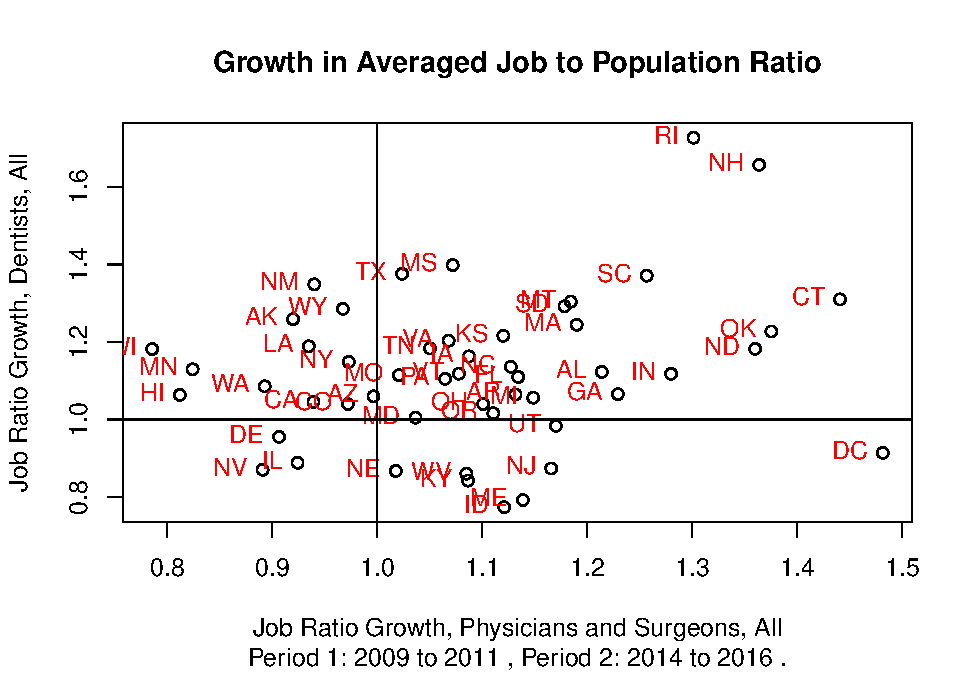
\includegraphics{BLS_Graphic_Reproduction_files/figure-latex/unnamed-chunk-4-1.pdf}

For example, the function above plot job growth rate of dentists over
job growth rate of physicians and surgeons. The first and second
occupations can take from the following:

\begin{Shaded}
\begin{Highlighting}[]
\FunctionTok{unique}\NormalTok{(}\FunctionTok{factor}\NormalTok{(Employment\_Data}\SpecialCharTok{$}\NormalTok{job\_type))}
\end{Highlighting}
\end{Shaded}

\begin{verbatim}
## [1] Dental Hygienists                           
## [2] Dentists, All                               
## [3] Nurses                                      
## [4] Physicians and Surgeons, All                
## [5] Physicians and Surgeons, Family Practitioner
## [6] Dentists, General                           
## 6 Levels: Dental Hygienists Dentists, All Dentists, General ... Physicians and Surgeons, Family Practitioner
\end{verbatim}

Here are some notes:

\begin{quote}
\begin{quote}
Use the exact name, as characters, for function input.
\end{quote}
\end{quote}

\begin{quote}
\begin{quote}
Dentists, All are calculated from summing up ALL dentist subcategories
(dentists, general; dental surgeons; etc.)
\end{quote}
\end{quote}

\begin{quote}
\begin{quote}
Dentists, General refers to denetists who does not specialize in surgeon
or other field. They are NOT found in original BLS data beofre 2003,
instead only Dentists\_All were found.
\end{quote}
\end{quote}

\begin{quote}
\begin{quote}
Similarly, Physicians and Surgeons, All were sum of all doctors,
phycisians, surgeons, etc.
\end{quote}
\end{quote}

\begin{quote}
\begin{quote}
See \url{https://www.bls.gov/oes/current/oes_stru.htm}, 29-1060,
29-1020, 29-2021, 29-1141 for more specific information.
\end{quote}
\end{quote}

The begin\_year\_1, end\_year\_1, begin\_year\_2, and end\_year\_2
parameter is by default 2009, 2011, 2014, and 2016 respectively, thus we
compare period between 2009 and 2011 with period between 2014 and 2016,
beginning and ending included. You can change it for other years.

plot is by default 1 so you get output plot. Set it to anything else for
no plot. give\_processed\_data was by default 0, set it to 1 to get
processed dataframe used for plotting.

\hypertarget{plot-with-bls-codes-for-occupations}{%
\subsection{Plot with BLS codes for
occupations}\label{plot-with-bls-codes-for-occupations}}

Alternatively, the following function takes number instead of occupation
names. It serves generally the same use:

\begin{Shaded}
\begin{Highlighting}[]
\NormalTok{Ratio\_Extractor\_by\_Code }\OtherTok{=} \ControlFlowTok{function}\NormalTok{(First\_Occupation\_Code, Second\_Occupation\_Code, Input\_Data,  }
                                   \AttributeTok{Begin\_Year\_1 =} \DecValTok{2009}\NormalTok{, }\AttributeTok{End\_Year\_1 =} \DecValTok{2011}\NormalTok{,}
                                   \AttributeTok{Begin\_Year\_2 =} \DecValTok{2014}\NormalTok{, }\AttributeTok{End\_Year\_2 =} \DecValTok{2016}\NormalTok{,}
                                   \AttributeTok{plot =} \DecValTok{1}\NormalTok{, }\AttributeTok{give\_processed\_data =} \DecValTok{0}\NormalTok{)\{}
  \CommentTok{\# This function basically does the same thing as above (Ratio\_Extractor),}
  \CommentTok{\# But it uses occupation code instead of occupation titles}
  \FunctionTok{return}\NormalTok{(}
    \FunctionTok{Ratio\_Extractor}\NormalTok{(}
      \AttributeTok{First\_Occupation =}\NormalTok{ Input\_Data[Input\_Data}\SpecialCharTok{$}\NormalTok{occ\_code }\SpecialCharTok{==}\NormalTok{ First\_Occupation\_Code, ][}\DecValTok{1}\NormalTok{, ]}\SpecialCharTok{$}\NormalTok{job\_type,}
      
      \DocumentationTok{\#\#\#\# This line shall be read as the following: For the lines in input\_data,}
      \DocumentationTok{\#\#\# With same occ\_code as the First Occupation Code input of the function,}
      \DocumentationTok{\#\#\# Take their first line, and the entry in "job\_type" variable}
      \DocumentationTok{\#\#\# This shall give occupation name by character to be used in}
      \DocumentationTok{\#\#\# Ratio\_Extractor function as written above.}
      
      \AttributeTok{Second\_Occupation =}\NormalTok{ Input\_Data[Input\_Data}\SpecialCharTok{$}\NormalTok{occ\_code }\SpecialCharTok{==}\NormalTok{ Second\_Occupation\_Code, ][}\DecValTok{1}\NormalTok{, ]}\SpecialCharTok{$}\NormalTok{job\_type,}
      
      \AttributeTok{Input\_Data =}\NormalTok{ Input\_Data, }
      \AttributeTok{Begin\_Year\_1 =}\NormalTok{ Begin\_Year\_1, }\AttributeTok{End\_Year\_1 =}\NormalTok{ End\_Year\_1,}
      \AttributeTok{Begin\_Year\_2 =}\NormalTok{ Begin\_Year\_2, }\AttributeTok{End\_Year\_2 =}\NormalTok{ End\_Year\_2,}
      \AttributeTok{plot =}\NormalTok{ plot, }\AttributeTok{give\_processed\_data =}\NormalTok{ give\_processed\_data}
      
      \DocumentationTok{\#\#\# All other parameters were passed without changes.}
\NormalTok{    )}
\NormalTok{  )}
\NormalTok{\}}
\end{Highlighting}
\end{Shaded}

To replicate the same plot as above, the following input were used:

\begin{Shaded}
\begin{Highlighting}[]
\FunctionTok{Ratio\_Extractor\_by\_Code}\NormalTok{(}\AttributeTok{First\_Occupation\_Code =} \DecValTok{1060}\NormalTok{, }
                        \AttributeTok{Second\_Occupation\_Code =} \DecValTok{1020}\NormalTok{, }
                        \AttributeTok{Input\_Data =}\NormalTok{ Employment\_Data)}
\end{Highlighting}
\end{Shaded}

\begin{verbatim}
## `summarise()` has grouped output by 'st', 'job_type'. You can override using
## the `.groups` argument.
\end{verbatim}

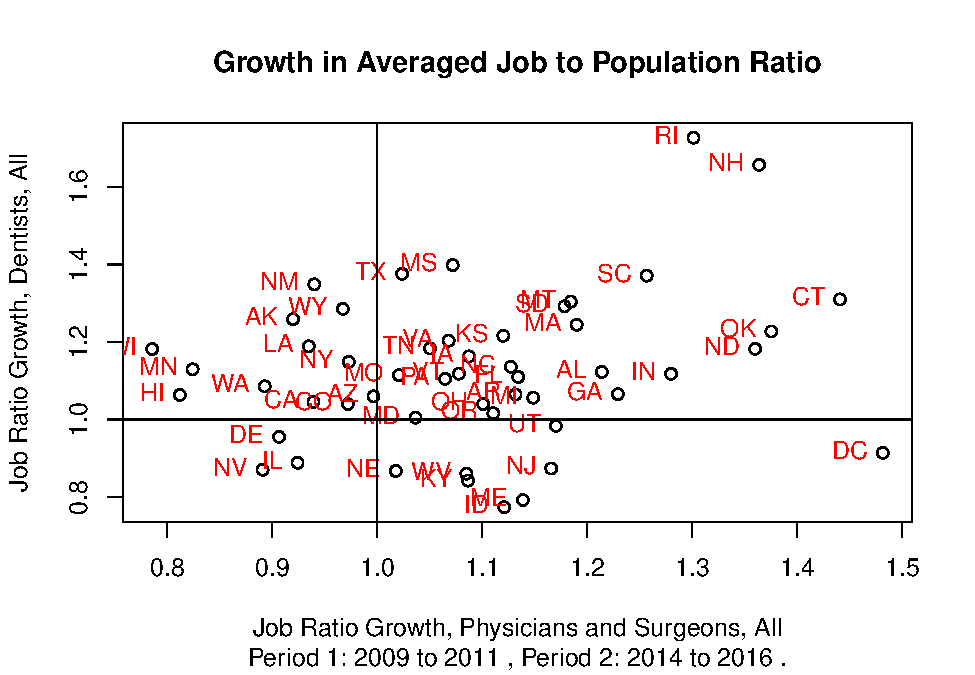
\includegraphics{BLS_Graphic_Reproduction_files/figure-latex/unnamed-chunk-7-1.pdf}

Since 29-1060 were BLS code for physicians and surgeons, and 1020 for
all dentists. Here is a table for job types along their codes:

\begin{Shaded}
\begin{Highlighting}[]
\FunctionTok{unique}\NormalTok{(Employment\_Data[, }\FunctionTok{c}\NormalTok{(}\StringTok{"job\_type"}\NormalTok{, }\StringTok{"occ\_code"}\NormalTok{)])}
\end{Highlighting}
\end{Shaded}

\begin{verbatim}
##                                          job_type occ_code
## 1                               Dental Hygienists     2021
## 2                                   Dentists, All     1020
## 3                                          Nurses     1141
## 4                    Physicians and Surgeons, All     1060
## 187  Physicians and Surgeons, Family Practitioner     1062
## 1448                            Dentists, General     1021
\end{verbatim}

The second row, occ\_code, are codes used as input for
Ratio\_Extractor\_by\_Code. To search for corresponding occupation and
their profile, description etc. on BLS website, add 29- before the code.

\hypertarget{plot-job-ratio-against-wage}{%
\subsection{Plot job ratio against
wage}\label{plot-job-ratio-against-wage}}

The following function make a scatterplot for datapoints representing 50
U.S. States and District Columbia. The X-axis is
job-per-1,000-population, or ave\_job\_ratio, or averaged jobs per 1,000
people over a period of years, for one occupation. The Y-axis is average
annual wage for one occupation, calculated as mean annual income of an
occpuation averaged over years. Not inflation adjusted.

These two occupations NEED NOT to be the same. Furthermore, their
beginning and ending years for averaging can also be self-defined and
need also not be the same.

Here is the list of input variable explained.

\begin{quote}
\begin{quote}
Occupation\_for\_Ratio: Name of the occupation for job/population ratio,
on X-axis
\end{quote}
\end{quote}

\begin{quote}
\begin{quote}
Occupation\_for\_Wage: Name of the occupation for average annual income,
on Y-axis. By default same as Occupation\_for\_Ratio but can be changed
\end{quote}
\end{quote}

\begin{quote}
\begin{quote}
Input\_Data: just use employment\_data
\end{quote}
\end{quote}

\begin{quote}
\begin{quote}
Begin\_Year\_Ratio, End\_Year\_Ratio: Defines year period to calculate
averaged job/population ratio. Default 2003 and 2018 respectively
\end{quote}
\end{quote}

\begin{quote}
\begin{quote}
Begin\_Year\_Wage, End\_Year\_Wage: Defines year period to calculate
averaged Annual Income. Default 2003 and 2018 respectively
\end{quote}
\end{quote}

\begin{quote}
\begin{quote}
plot: 1 if you need scatterplot output, default 1
\end{quote}
\end{quote}

\begin{quote}
\begin{quote}
give\_processed\_data: 1 if you need processed data frame used for
plotting to be returned. Default 0.
\end{quote}
\end{quote}

Specific technical details are in comments in code below:

\begin{Shaded}
\begin{Highlighting}[]
\NormalTok{Ratio\_Wage\_Extractor }\OtherTok{=} \ControlFlowTok{function}\NormalTok{(Occupation\_for\_Ratio, }
                                \AttributeTok{Occupation\_for\_Wage =}\NormalTok{ Occupation\_for\_Ratio, }
\NormalTok{                                Input\_Data,  }
                           \AttributeTok{Begin\_Year\_Ratio =} \DecValTok{2003}\NormalTok{, }\AttributeTok{End\_Year\_Ratio =} \DecValTok{2018}\NormalTok{,}
                           \AttributeTok{Begin\_Year\_Wage =} \DecValTok{2003}\NormalTok{, }\AttributeTok{End\_Year\_Wage =} \DecValTok{2018}\NormalTok{,}
                           \AttributeTok{plot =} \DecValTok{1}\NormalTok{, }\AttributeTok{give\_processed\_data =} \DecValTok{0}\NormalTok{)\{}
  
\NormalTok{  temp }\OtherTok{=}\NormalTok{ Input\_Data}
\NormalTok{  temp }\OtherTok{=}\NormalTok{ temp[temp}\SpecialCharTok{$}\NormalTok{st }\SpecialCharTok{!=} \StringTok{"PR"}\NormalTok{, ]}
  \DocumentationTok{\#\# Input data and drop Puerto Rico}
  
\NormalTok{  data\_for\_ratio }\OtherTok{=}\NormalTok{ temp }\SpecialCharTok{\%\textgreater{}\%} \FunctionTok{filter}\NormalTok{(job\_type }\SpecialCharTok{==}\NormalTok{ Occupation\_for\_Ratio) }\SpecialCharTok{\%\textgreater{}\%} 
    
    \DocumentationTok{\#\#\#\# This filters the entries with correct occupation}
    \DocumentationTok{\#\#\#\# to calculate job/population ratio, A.K.A. ave\_job\_ratio}
    
    \FunctionTok{filter}\NormalTok{(year }\SpecialCharTok{\textgreater{}=}\NormalTok{ Begin\_Year\_Ratio }\SpecialCharTok{\&}\NormalTok{ year }\SpecialCharTok{\textless{}=}\NormalTok{ End\_Year\_Ratio) }\SpecialCharTok{\%\textgreater{}\%}
    
    \CommentTok{\# Filter year range}
    
    \FunctionTok{filter}\NormalTok{(}\SpecialCharTok{!}\FunctionTok{is.na}\NormalTok{(Est\_Population)) }\SpecialCharTok{\%\textgreater{}\%} \FunctionTok{filter}\NormalTok{(tot\_employment }\SpecialCharTok{\textgreater{}} \DecValTok{0}\NormalTok{)}
    \DocumentationTok{\#\# Drop useless entries. Same idea as previous function}
  
  \CommentTok{\#Group them and sum \textquotesingle{}em up}
\NormalTok{  data\_for\_ratio }\OtherTok{=}\NormalTok{ data\_for\_ratio }\SpecialCharTok{\%\textgreater{}\%} \FunctionTok{group\_by}\NormalTok{(st) }\SpecialCharTok{\%\textgreater{}\%}
    \FunctionTok{summarize}\NormalTok{(}\AttributeTok{ave\_job\_ratio =} \FunctionTok{sum}\NormalTok{(tot\_employment) }\SpecialCharTok{/} \FunctionTok{sum}\NormalTok{(Est\_Population)) }\SpecialCharTok{\%\textgreater{}\%}
    \FunctionTok{mutate}\NormalTok{(}\AttributeTok{ave\_job\_ratio =}\NormalTok{ ave\_job\_ratio }\SpecialCharTok{*} \DecValTok{1000}\NormalTok{) }\SpecialCharTok{\%\textgreater{}\%}
    \FunctionTok{unique}\NormalTok{()}
  
  \DocumentationTok{\#\#\# The above function groups the data by state and find job ratio}
  \DocumentationTok{\#\#\# Through sum(tot\_employment) / sum(Est\_Population).}
  \DocumentationTok{\#\#\# This might involve replicate calculations for all years. However, }
  \DocumentationTok{\#\#\# This is a small dataset so the calculation time is ignorable.}
  
  \CommentTok{\#Compute mean wage.}
\NormalTok{  data\_for\_wage }\OtherTok{=}\NormalTok{ temp }\SpecialCharTok{\%\textgreater{}\%} \FunctionTok{filter}\NormalTok{(job\_type }\SpecialCharTok{==}\NormalTok{ Occupation\_for\_Wage) }\SpecialCharTok{\%\textgreater{}\%}
    
    \DocumentationTok{\#\# Similarly, filter only those occupation used}
    \DocumentationTok{\#\#\# to calculate wages.}
    
    \FunctionTok{filter}\NormalTok{(year }\SpecialCharTok{\textgreater{}=}\NormalTok{ Begin\_Year\_Wage }\SpecialCharTok{\&}\NormalTok{ year }\SpecialCharTok{\textless{}=}\NormalTok{ End\_Year\_Wage) }\SpecialCharTok{\%\textgreater{}\%}
    
    \DocumentationTok{\#\# Year range}
    
    \FunctionTok{filter}\NormalTok{(}\SpecialCharTok{!}\FunctionTok{is.na}\NormalTok{(Est\_Population)) }\SpecialCharTok{\%\textgreater{}\%} \FunctionTok{filter}\NormalTok{(tot\_employment }\SpecialCharTok{\textgreater{}} \DecValTok{0}\NormalTok{)}
  
\NormalTok{  data\_for\_wage }\OtherTok{=}\NormalTok{ data\_for\_wage }\SpecialCharTok{\%\textgreater{}\%} \FunctionTok{group\_by}\NormalTok{(st) }\SpecialCharTok{\%\textgreater{}\%}
    \FunctionTok{summarize}\NormalTok{(}\AttributeTok{ave\_annual\_wage =} \FunctionTok{mean}\NormalTok{(annual\_mean\_income, }\AttributeTok{na.rm =} \ConstantTok{TRUE}\NormalTok{)) }\SpecialCharTok{\%\textgreater{}\%}
    \FunctionTok{mutate}\NormalTok{(}\AttributeTok{ave\_annual\_wage =}\NormalTok{ ave\_annual\_wage }\SpecialCharTok{/} \DecValTok{1000}\NormalTok{) }\SpecialCharTok{\%\textgreater{}\%}
    \FunctionTok{unique}\NormalTok{()}
  
  \DocumentationTok{\#\# Again, by each state make average on mean annual income}
  
\NormalTok{  temp }\OtherTok{=} \FunctionTok{merge}\NormalTok{(data\_for\_ratio, data\_for\_wage, }\AttributeTok{by =} \StringTok{"st"}\NormalTok{)}
  
  \ControlFlowTok{if}\NormalTok{(plot }\SpecialCharTok{==} \DecValTok{1}\NormalTok{)\{}
    \FunctionTok{plot}\NormalTok{(}\AttributeTok{x =}\NormalTok{ temp}\SpecialCharTok{$}\NormalTok{ave\_job\_ratio, }\AttributeTok{y =}\NormalTok{ temp}\SpecialCharTok{$}\NormalTok{ave\_annual\_wage,}
         \AttributeTok{xlab =} \FunctionTok{paste}\NormalTok{(}\StringTok{"Averaged job per 1,000 People, "}\NormalTok{, }
\NormalTok{                      Occupation\_for\_Ratio, }\AttributeTok{sep =} \StringTok{""}\NormalTok{),}
         \AttributeTok{ylab =} \FunctionTok{paste}\NormalTok{(}\StringTok{"Averaged yearly earning of "}\NormalTok{, }
\NormalTok{                      Occupation\_for\_Wage, }\StringTok{", in 1,000 dollars"}\NormalTok{, }\AttributeTok{sep =} \StringTok{""}\NormalTok{))}
    \CommentTok{\# Fix Scale)}
    \FunctionTok{title}\NormalTok{(}\AttributeTok{main =} \StringTok{"Yearly Earning (in thousands of dollars) }
\StringTok{          over Job per 1,000 people"}\NormalTok{,}
          \AttributeTok{sub =} \FunctionTok{paste}\NormalTok{(}\StringTok{"Period for X{-}axis:"}\NormalTok{, Begin\_Year\_Ratio, }
                      \StringTok{"to"}\NormalTok{, End\_Year\_Ratio, }
                      \StringTok{", Period for Y{-}axis:"}\NormalTok{, Begin\_Year\_Wage, }
                      \StringTok{"to"}\NormalTok{, End\_Year\_Wage, }\StringTok{"."}\NormalTok{))}
    \FunctionTok{text}\NormalTok{(temp[, }\DecValTok{2}\NormalTok{], temp[, }\DecValTok{3}\NormalTok{], temp[, }\DecValTok{1}\NormalTok{], }\AttributeTok{pos =} \DecValTok{2}\NormalTok{, }\AttributeTok{col =} \StringTok{"red"}\NormalTok{)}
\NormalTok{  \}}
  \ControlFlowTok{if}\NormalTok{(give\_processed\_data }\SpecialCharTok{==} \DecValTok{1}\NormalTok{)\{}
    \FunctionTok{return}\NormalTok{(temp)}
\NormalTok{  \}}
\NormalTok{\}}
\end{Highlighting}
\end{Shaded}

Similarly, here is a function that allows plotting with code, using same
occupation title to code format as in ratio\_extractor function.

\begin{Shaded}
\begin{Highlighting}[]
\NormalTok{Ratio\_Wage\_Extractor\_by\_Code }\OtherTok{=} \ControlFlowTok{function}\NormalTok{(Occupation\_for\_Ratio\_Code, }
                                        \AttributeTok{Occupation\_for\_Wage\_Code =}\NormalTok{ Occupation\_for\_Ratio\_Code,}
\NormalTok{                                        Input\_Data,  }
                                        \AttributeTok{Begin\_Year\_Ratio =} \DecValTok{2003}\NormalTok{, }\AttributeTok{End\_Year\_Ratio =} \DecValTok{2018}\NormalTok{,}
                                        \AttributeTok{Begin\_Year\_Wage =} \DecValTok{2003}\NormalTok{, }\AttributeTok{End\_Year\_Wage =} \DecValTok{2018}\NormalTok{,}
                                        \AttributeTok{plot =} \DecValTok{1}\NormalTok{, }\AttributeTok{give\_processed\_data =} \DecValTok{0}\NormalTok{)\{}
  \FunctionTok{return}\NormalTok{(}
    \FunctionTok{Ratio\_Wage\_Extractor}\NormalTok{(}
      \AttributeTok{Occupation\_for\_Ratio =}\NormalTok{ Input\_Data[Input\_Data}\SpecialCharTok{$}\NormalTok{occ\_code }\SpecialCharTok{==}\NormalTok{ Occupation\_for\_Ratio\_Code, ][}\DecValTok{1}\NormalTok{, ]}\SpecialCharTok{$}\NormalTok{job\_type,}
      \AttributeTok{Occupation\_for\_Wage =}\NormalTok{ Input\_Data[Input\_Data}\SpecialCharTok{$}\NormalTok{occ\_code }\SpecialCharTok{==}\NormalTok{ Occupation\_for\_Wage\_Code, ][}\DecValTok{1}\NormalTok{, ]}\SpecialCharTok{$}\NormalTok{job\_type,}
      \AttributeTok{Input\_Data =}\NormalTok{ Input\_Data, }
      \AttributeTok{Begin\_Year\_Ratio =}\NormalTok{ Begin\_Year\_Ratio, }\AttributeTok{End\_Year\_Ratio =}\NormalTok{ End\_Year\_Ratio,}
      \AttributeTok{Begin\_Year\_Wage =}\NormalTok{ Begin\_Year\_Wage, }\AttributeTok{End\_Year\_Wage =}\NormalTok{ End\_Year\_Wage,}
      \AttributeTok{plot =}\NormalTok{ plot, }\AttributeTok{give\_processed\_data =}\NormalTok{ give\_processed\_data}
\NormalTok{    )}
\NormalTok{  )}
\NormalTok{\}}
\end{Highlighting}
\end{Shaded}

Here is an example with dentists\_all

\begin{Shaded}
\begin{Highlighting}[]
\FunctionTok{Ratio\_Wage\_Extractor\_by\_Code}\NormalTok{(}\AttributeTok{Occupation\_for\_Ratio\_Code =} \DecValTok{1020}\NormalTok{, }\AttributeTok{Input\_Data =}\NormalTok{ Employment\_Data)}
\end{Highlighting}
\end{Shaded}

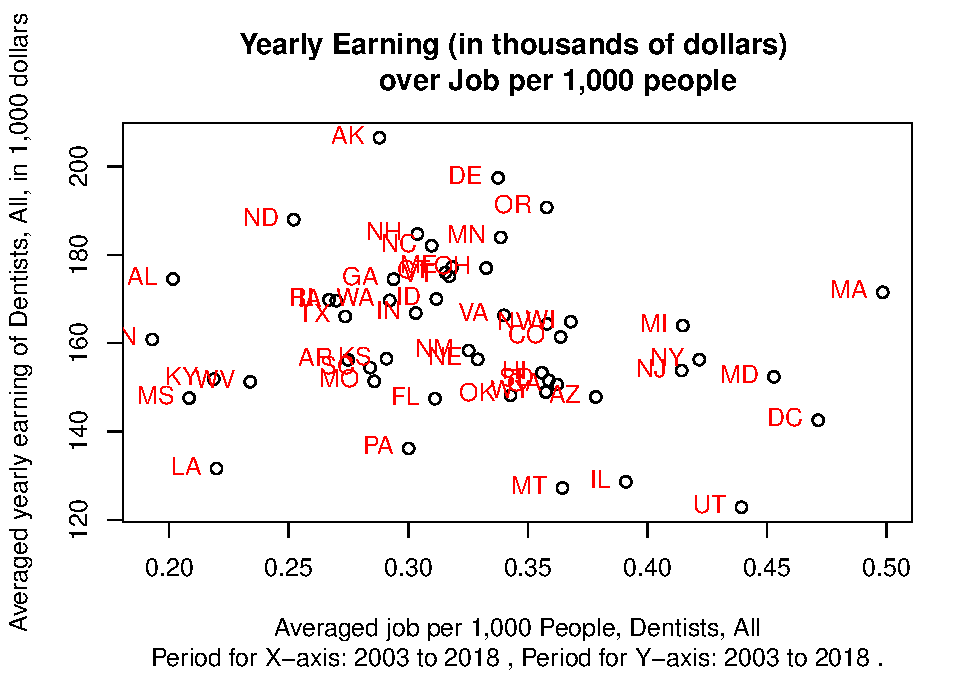
\includegraphics{BLS_Graphic_Reproduction_files/figure-latex/unnamed-chunk-11-1.pdf}

You can create more plots with these functions should you like.

\end{document}
